%%
%% This is file `sample-authordraft.tex',
%% generated with the docstrip utility.
%%
%% The original source files were:
%%
%% samples.dtx  (with options: `authordraft')
%% 
%% IMPORTANT NOTICE:
%% 
%% For the copyright see the source file.
%% 
%% Any modified versions of this file must be renamed
%% with new filenames distinct from sample-authordraft.tex.
%% 
%% For distribution of the original source see the terms
%% for copying and modification in the file samples.dtx.
%% 
%% This generated file may be distributed as long as the
%% original source files, as listed above, are part of the
%% same distribution. (The sources need not necessarily be
%% in the same archive or directory.)
%%
%% Commands for TeXCount
%TC:macro \cite [option:text,text]
%TC:macro \citep [option:text,text]
%TC:macro \citet [option:text,text]
%TC:envir table 0 1
%TC:envir table* 0 1
%TC:envir tabular [ignore] word
%TC:envir displaymath 0 word
%TC:envir math 0 word
%TC:envir comment 0 0
%%
%%
%% The first command in your LaTeX source must be the \documentclass command.
\documentclass[sigconf,anonymous]{acmart}
\usepackage{multirow}
\graphicspath{ {./images/} }
%% NOTE that a single column version may required for 
%% submission and peer review. This can be done by changing
%% the \doucmentclass[...]{acmart} in this template to 
%% \documentclass[manuscript,screen]{acmart}
%% 
%% To ensure 100% compatibility, please check the white list of
%% approved LaTeX packages to be used with the Master Article Template at
%% https://www.acm.org/publications/taps/whitelist-of-latex-packages 
%% before creating your document. The white list page provides 
%% information on how to submit additional LaTeX packages for 
%% review and adoption.
%% Fonts used in the template cannot be substituted; margin 
%% adjustments are not allowed.

%%
%% \BibTeX command to typeset BibTeX logo in the docs
\AtBeginDocument{%
  \providecommand\BibTeX{{%
    \normalfont B\kern-0.5em{\scshape i\kern-0.25em b}\kern-0.8em\TeX}}}

%% Rights management information.  This information is sent to you
%% when you complete the rights form.  These commands have SAMPLE
%% values in them; it is your responsibility as an author to replace
%% the commands and values with those provided to you when you
%% complete the rights form.
%% TODO: Fill in copyright info and uncomment
% \setcopyright{acmcopyright}
% \copyrightyear{2018}
% \acmYear{2018}
% \acmDOI{XXXXXXX.XXXXXXX}

\acmYear{2023}
\acmConference[ACE '23]{ACE 2023: Proceedings of the Twenty-Fifth Australasian Computing Education Conference}{30 Jan--3 Feb,
  2023}{Melbourne, VIC, Australia}

 
%% These commands are for a PROCEEDINGS abstract or paper.
% TODO: Fill in and uncomment
% \acmConference[Conference acronym 'XX]{Make sure to enter the correct
%   conference title from your rights confirmation emai}{June 03--05,
%   2018}{Woodstock, NY}
%
%  Uncomment \acmBooktitle if th title of the proceedings is different
%  from ``Proceedings of ...''!
%
%\acmBooktitle{Woodstock '18: ACM Symposium on Neural Gaze Detection,
%  June 03--05, 2018, Woodstock, NY}
% TODO: Fill in and uncomment
% \acmPrice{15.00}
% \acmISBN{978-1-4503-XXXX-X/18/06}


%%
%% Submission ID.
%% Use this when submitting an article to a sponsored event. You'll
%% receive a unique submission ID from the organizers
%% of the event, and this ID should be used as the parameter to this command.
%%\acmSubmissionID{123-A56-BU3}

%%
%% For managing citations, it is recommended to use bibliography
%% files in BibTeX format.
%%
%% You can then either use BibTeX with the ACM-Reference-Format style,
%% or BibLaTeX with the acmnumeric or acmauthoryear sytles, that include
%% support for advanced citation of software artefact from the
%% biblatex-software package, also separately available on CTAN.
%%
%% Look at the sample-*-biblatex.tex files for templates showcasing
%% the biblatex styles.
%%

%%
%% For managing citations, it is recommended to use bibliography
%% files in BibTeX format.
%%
%% You can then either use BibTeX with the ACM-Reference-Format style,
%% or BibLaTeX with the acmnumeric or acmauthoryear sytles, that include
%% support for advanced citation of software artefact from the
%% biblatex-software package, also separately available on CTAN.
%%
%% Look at the sample-*-biblatex.tex files for templates showcasing
%% the biblatex styles.
%%

%%
%% The majority of ACM publications use numbered citations and
%% references.  The command \citestyle{authoryear} switches to the
%% "author year" style.
%%
%% If you are preparing content for an event
%% sponsored by ACM SIGGRAPH, you must use the "author year" style of
%% citations and references.
%% Uncommenting
%% the next command will enable that style.
%%\citestyle{acmauthoryear}

%%
%% end of the preamble, start of the body of the document source.
\begin{document}

%%
%% The "title" command has an optional parameter,
%% allowing the author to define a "short title" to be used in page headers.
\title{Metacodenition: A Tool to Scaffold the Problem-Solving Process for Novice Programmers}

%%
%% The "author" command and its associated commands are used to define
%% the authors and their affiliations.
%% Of note is the shared affiliation of the first two authors, and the
%% "authornote" and "authornotemark" commands
%% used to denote shared contribution to the research.
\author{Yulia Pechorina}
\affiliation{%
  \institution{The University of Auckland}
  \city{Auckland}
  \country{New Zealand}}
\email{ypec413@aucklanduni.ac.nz}

\author{Keith Anderson}
\affiliation{%
  \institution{The University of Auckland}
  \city{Auckland}
  \country{New Zealand}}
\email{kand198@aucklanduni.ac.nz}

\author{Paul Denny}
\affiliation{%
  \institution{The University of Auckland}
  \city{Auckland}
  \country{New Zealand}}
\email{p.denny@auckland.ac.nz}

%%
%% By default, the full list of authors will be used in the page
%% headers. Often, this list is too long, and will overlap
%% other information printed in the page headers. This command allows
%% the author to define a more concise list
%% of authors' names for this purpose.
\renewcommand{\shortauthors}{Pechorina, Anderson, and Denny}
\renewcommand{\sectionautorefname}{Section}
\renewcommand{\subsectionautorefname}{Section}
\renewcommand{\subsubsectionautorefname}{Section}

%%
%% The abstract is a short summary of the work to be presented in the
%% article.
\begin{abstract}
    More novices  are taking introductory programming courses today than ever. While most programming-related skills are taught explicitly in these courses, it is common for problem-solving to be taught implicitly – usually through having students perform programming drills. This can lead to students not developing the required problem-solving skills for success, manifesting in students feeling lost when solving problems with no idea how to progress. A substantial body of work has investigated the explicit teaching of problem-solving and related metacognitive skills. This previous work has shown that teaching students a model for the problem-solving process and how to track their progress along it leads to greater self-efficacy and productivity. Studies have shown that interventions targeting isolated steps in these models are effective, but there have been few efforts to combine these into a single coherent tool. Our contribution is a novel tool called Metacodenition, which provides metacognitive scaffolding for an existing problem-solving framework. Our evaluation shows that Metacodenition’s scaffolding improves performance on code-writing tasks and students view Metacodenition to be a helpful tool they would use voluntarily.
\end{abstract}

%%
%% The code below is generated by the tool at http://dl.acm.org/ccs.cfm.
%% Please copy and paste the code instead of the example below.
%%
\begin{CCSXML}
<ccs2012>
   <concept>
       <concept_id>10003456.10003457.10003527</concept_id>
       <concept_desc>Social and professional topics~Computing education</concept_desc>
       <concept_significance>500</concept_significance>
   </concept>
   <concept>
        <concept_id>10010405.10010489.10010491</concept_id>
        <concept_desc>Applied computing~Interactive learning environments</concept_desc>
        <concept_significance>500</concept_significance>
    </concept>
 </ccs2012>
\end{CCSXML}

\ccsdesc[500]{Social and professional topics~Computing education}
\ccsdesc[500]{Applied computing~Interactive learning environments}

%%
%% Keywords. The author(s) should pick words that accurately describe
%% the work being presented. Separate the keywords with commas.
\keywords{metacognition, problem-solving, software engineering education, programming education, novice programmers}

% TODO: fill and uncomment if necessary
% \received{20 February 2007}
% \received[revised]{12 March 2009}
% \received[accepted]{5 June 2009}

%%
%% This command processes the author and affiliation and title
%% information and builds the first part of the formatted document.
\maketitle

\section{Introduction} \label{sec:introduction}
Learning to program requires students to develop several skills, one of which is problem-solving \cite{lakanen2015, bruce2003}. It is widely accepted that problem-solving is both a critical skill \cite{gomes2007}, and one of the most difficult skills for novices to develop \cite{medeiros2019}. Further, an ITiCSE working group study found that many students in introductory programming courses lacked effective problem-solving skills \cite{lister2004}.

One factor explaining poor problem-solving skills in novices is the curriculum of introductory programming courses. Programming skills taught in introductory programming courses can be divided into programming knowledge and programming problem-solving strategies. Programming knowledge refers to the syntax and semantics of a language, whereas programming problem-solving strategies refer to how one applies programming knowledge to solve a problem \cite{deraat2009}. In a typical course curriculum, programming knowledge is explicitly taught, whereas problem-solving strategies are often implicitly taught \cite{luxtonreilly2018}. One example of a curriculum that aims to explicitly teach problem-solving strategies is \emph{How to Design Programs}, which introduces a six-step process for designing a program from a problem statement \cite{felleisen2001}.

However, even when problem-solving strategies are explicitly taught, novice programmers often face difficulties learning problem-solving because they lack metacognitive awareness \cite{anneli1993, loksa2016, mani2013}. Metacognitive awareness refers to being aware of one's own thinking and problem-solving strategies \cite{gibson1996}, and plays a significant role in programming \cite{parham2010}. When programming, students use metacognition to move between the steps of a problem-solving process and decide when to revisit steps \cite{parham2010}. Interest in applying theories of metacognition and self-regulation to computer programming education has increased in recent years \cite{loksa2022}. For practitioners, this presents an opportunity to take theories from education research within and outside of computer programming and apply them in the classroom.

While increased interest in this area has led to more publications in recent years \cite{loksa2022}, most prior work has focused on problem-solving interventions that target one step of a problem-solving framework at a time. This makes it difficult to apply research findings to how we teach novices to program. There is a need for easy-to-use tools which combine multiple interventions from the literature and provide explicit guidance to students throughout the problem-solving process, enabling them to develop their metacognitive skills.

Our contribution is an integrated development environment (IDE) called Metacodenition, designed to provide metacognitive scaffolding during code writing exercises. We outline the design of Metacodenition and then evaluate its effectiveness through a study involving 821 first-year engineering students taking an introductory programming course. We investigate the following research questions:

\begin{itemize}
\item[\textbf{RQ1:}]  What are students' perceptions toward using Metacodenition for problem-solving activities?
\item[\textbf{RQ2:}]  Does the scaffolding provided by Metacodenition improve performance on code-writing tasks?
\end{itemize}


The remainder of this paper is organised as follows. \autoref{sec:relatedwork} reviews related work on strategies, frameworks, and interventions designed to aid novices in developing problem-solving skills. In \autoref{sec:design}, we present our approach to designing Metacodenition. We evaluate the tool by analysing student feedback and the correctness of submitted code in \autoref{sec:evaluation}. The results and discussion of this evaluation are reported in \autoref{sec:results}, and we present conclusions in \autoref{sec:conclusion}.

\section{Related Work} \label{sec:relatedwork}

\subsection{Problem-solving frameworks} \label{sec:relatedwork-frameworks}
Loksa et al. \cite{loksa20162} developed a programming-specific problem-solving framework consisting of the following stages: (1) reinterpreting the problem prompt, (2) searching for analogous problems, (3) searching for solutions, (4) evaluating a potential solution, (5) implementing a solution, and (6) evaluating an implemented solution (see \autoref{tab:loksaFramework}).

\begin{table}
  \caption{Loksa et al.'s problem-solving stages \cite{loksa20162}}
  \label{tab:loksaFramework}
  \begin{tabular}{c|p{35mm}|p{35mm}}
    \toprule
    \#&Stage&Description\\
    \midrule
    1&Reinterpreting the problem prompt&Understanding and interpreting the problem statement and requirements\\
    \midrule
    2&Searching for analogous problems&Drawing upon previously encountered problems \\
    \midrule
    3&Searching for solutions&Seeking solutions that will solve the problem\\
    \midrule
    4&Evaluating a potential solution&Evaluating whether the solution meets problem requirements, often using prototyping techniques such as pseudo code\\
    \midrule
    5&Implementing a solution&Writing the solution code \\
    \midrule
    6&Evaluating an implemented solution&Evaluating whether the current solution meets the problem requirements, usually through testing and debugging\\
    \bottomrule
  \end{tabular}
\end{table}

Along with the six stages, the authors also described four problem-solving interventions: (1) explicitly teaching the framework to students, (2) getting students to identify their current stage in the framework when asking for help, (3) a physical handout of the problem-solving process, (4) an idea garden in the students' IDE which contains ideas categorized by problem-solving stage. This approach was successful at increasing students' productivity and self-efficacy.

“The Seven Steps” is a different framework with a strong focus on algorithmic problems developed by Hilton et al. \cite{hilton2019}. The framework consists of the following steps: (1) work an example yourself, (2) write down exactly what you just did, (3) generalize, (4) test your algorithm, (5) translate to code, and (6) test. These steps help students design and implement an algorithm to solve a solution. In their study, the authors found that graduate students had a higher engagement with the framework than undergraduate students, although found no significant relationship between student engagement and performance.

Another framework, described by the ITiCSE working group \cite{mccracken2001}, consists of the following steps: (1) abstract the problem from its description, (2) generate sub-problems, (3) transform sub-problems into sub-solutions, (4) re-compose, and (5) evaluate and iterate. The authors found that novices often skipped the early stages of the problem-solving process and attributed this to the heavy focus on the later stages of the problem-solving process.

Of these papers, only Loksa et al. provided an intervention within the students' learning environments in the form of an Idea Garden. However, not all stages were included, and the scaffolding for moving between the problem-solving stages and monitoring one's problem-solving state was provided externally via physical props.

We chose Loksa et al.'s problem-solving framework to guide our work as it is directly informed by the field of metacognition, is less algorithmic than Hilton et al.'s framework, and places more emphasis on early problem-solving stages than the ITiCSE framework. Many of the recent studies which investigate providing problem-solving and metacognitive interventions build on the work done by Loksa et al. These interventions aim to increase students' problem-solving and metacognitive performance at individual stages of the Loksa et al. framework. This provides an opportunity to design a tool that explicitly teaches the framework to students and builds on individual interventions from the literature. Such a tool could benefit from compounding the positive effects of individual interventions and increase the scalability of teaching students the framework. These existing studies are summarised in \autoref{tab:existingStudies}.

\begin{table*}
  \caption{Summary of existing Studies Mapped to Loksa et al.'s Framework.}
  \label{tab:existingStudies}
  \begin{tabular}{c c p{10em} c c p{22em}}
    \toprule
    Author&Step&Intervention&Participants&Year&Finding\\
    \midrule
    Prather et al. \cite{prather2019}&1& Solving test cases&36&2019&Students who solved tests cases prior to writing code made fewer errors.\\
    \midrule
    Denny et al. \cite{denny2019}&1&Solving test cases&976&2019&Students who solved tests cases prior to writing code made fewer errors.\\
    \midrule
    Craig et al. \cite{craig2019}&1&Solving test cases&831&2019&The effectiveness of solving a test case before programming is dependent on the complexity problem being solved.\\
    \midrule
    Janzen et al. \cite{janzen2008}&1, 6&Writing test cases&140&2008&Writing test-cases before code increased assessment scores and decreased time spent.\\
    \midrule
    Weinman et al. \cite{weinman2021}&2&Faded Parsons problems&237&2021&Faded Parsons problems are an effective way to teach reusable programming patterns.\\
    \midrule
    Garcia \cite{garcia2021}&4&Design-level Parsons problems&10&2018&Parsons problems are effective in teaching students problem decomposition and solution design.\\
    \midrule
    Corno et al. \cite{corno2021}& 1, 3, 5&Decomposing a problem into sub-problems, linking sub-problems to code fragments, rearranging code fragments into a solution&N/A&2021&A pedagogic IDE can provide effective scaffolding for the problem-solving process.\\
    \midrule
    Prather et al. \cite{prather2017}&5&Enhanced compiler error messages&31&2017&Enhanced compiler error messages led to fewer incorrect answers in experimental group.\\
    \bottomrule
  \end{tabular}
\end{table*}

\subsection{Interventions related to ``Reinterpreting the problem prompt''} \label{sec:relatedwork-reinterpreting}
Much of the current body of work addresses the issue of problem comprehension, and this directly relates to the problem-solving stage of “reinterpreting the problem prompt”. Often, students misinterpret the problem prompt and answer the wrong question \cite{craig2019}. This is especially dangerous, as students risk becoming stuck and unable to progress towards a correct solution for the problem prompt until they attempt to “reinterpret the problem prompt” again \cite{prather2018}. Previous work has also found that students struggle to realize that they have misinterpreted the problem prompt \cite{prather2018,prather2019}. It is not uncommon for students to repeatedly misinterpret the problem prompt upon re-reading \cite{prather2019}.

Studies of interventions that aim to increase student problem comprehension typically involve test cases. These interventions can be divided into solving test cases (\autoref{sec:relatedwork-reinterpreting-solving}) and writing test cases (\autoref{sec:relatedwork-reinterpreting-writing}).

\subsubsection{Solving test cases} \label{sec:relatedwork-reinterpreting-solving}
Prather et al. \cite{prather2019}, Denny et al. \cite{denny2019}, and Craig et al. \cite{craig2019} have all investigated the effect metacognitive scaffolding has on student performance by having students solve test cases before coding.

Prather et al. found this led to faster task completion, a higher completion rate, and fewer attempts before completion \cite{prather2019}. In contrast, Denny et al. did not find any difference in completion time or the number of submissions but did find that the intervention decreased the number of errors students made \cite{denny2019}. Craig et al. found that the effectiveness of this intervention depended on the question type, being less effective for questions which primarily tested language or library knowledge \cite{craig2019}.

\subsubsection{Writing test cases} \label{sec:relatedwork-reinterpreting-writing}
A related approach of requiring students to write test-cases before they solve the problem, in the tradition of test-driven development (TDD), was taken by Janzen et al. \cite{janzen2008}. For a group of CS2 students, the authors found that students who wrote tests first achieved higher grades and spent less time writing the solution. However, they found no difference in the CS1 group who received the same intervention. This may indicate that a TDD approach is less suitable for novice programmers.

\subsection{Interventions related to ``Searching for analogous solutions''} \label{sec:relatedwork-searching}
Teaching reusable programming patterns can help a student build a bank of analogous problems to search for during this problem-solving stage. The use of Faded Parsons problems as a method to teach reusable programming patterns was investigated by Weinman et al. \cite{weinman2021}. Faded Parsons problems differ from standard Parsons problems by including blank spaces within the Parsons fragments, which the student must fill. The authors found that Faded Parsons problems were a successful intervention in teaching reusable programming patterns and are more popular than traditional code-writing exercises with students.

\subsection{Interventions related to ``Evaluating a potential solution''} \label{sec:relatedwork-evaluating}
Students often use prototyping techniques such as pseudo code to evaluate a potential solution. Parsons problems as a prototyping technique were investigated by Garcia \cite{garcia2021}. In this investigation, pieces of the high-level design of an algorithm were given to students in the form of a Parsons problem, and led to higher-quality final solutions from students. However, in this work the study size was relatively small.

\subsection{Interventions related to ``Implementing a solution''} \label{sec:relatedwork-implementing}
One of the very well known difficulties novices encounter when implementing their solutions is interpreting error messages \cite{becker2019compiler}. Prather et al. addressed this in a study on the helpfulness of \emph{enhanced compiler error messages}. The students in the experimental group received enhanced compiler error messages, where error messages had wording and structure better suited to novices. This led to significantly fewer incorrect answers. Students indicated that they believed the enhanced error messages were useful.

\subsection{Designing tools to support problem-solving} \label{sec:relatedwork-designing}
Sáenz and Russis investigated how ten novice students envision a tool to support their metacognitive awareness during problem-solving \cite{saenz2022}. From consulting directly with a group of students, the authors outlined several implications for designing a tool for supporting problem-solving strategies. These design implications included:
\begin{itemize}
    \item Supporting artefacts different from code

    \begin{itemize}
    \item
%    \begin{description}
        Generally, in programming assessments, only students' final code is assessed. Consequently, many novice students consider developing artefacts such as annotations or pseudo code a wasted effort, especially when time constrained. A tool should capture all other artefacts that students produce rather than just their final code.
    \end{itemize}

%    \end{description}
    \item Integrate and link the programming exercise text to the code constructs
    \begin{itemize}
    \item
%    \begin{description}
        Most students stated that they kept the problem description next to them while coding. Additionally, one student's sketch of a problem-solving tool showed the problem text placed next to their code. A tool should allow students to link fragments of the problem text to code constructs and create comments and annotations for these links.
    \end{itemize}
%    \end{description}
    \item Supporting the choice of algorithms and the data structure
    \begin{itemize}
    \item
%    \begin{description}
        Some students stated that their biggest challenge was choosing the correct algorithm and data structure for their solution. One student's sketch presented an area which provided documentation on various data structures.
    \end{itemize}
%    \end{description}
    \item Formatting and commenting features for the text and code
    \begin{itemize}
    \item
%    \begin{description}
       The most common problem-solving strategy described by students was highlighting keywords in the problem statement. A problem-solving tool should allow students to format the problem text, including highlighting or adding comments.
    \end{itemize}
%    \end{description}
\end{itemize}
These design implications directly informed our design choices when developing Metacodenition and are documented in \autoref{sec:design}.

\subsection{Tools for supporting problem-solving} \label{sec:relatedwork-tools}
To support problem-solving skills among novices, Corno et al. developed a tool called TextCode, which incorporates multiple problem-solving steps: understanding the problem before coding, decomposing the problem into sub-problems, solving each sub-problem individually, and arranging the solution to each sub-problem to build a general solution \cite{corno2021}. In Loksa et al.'s framework, these stages loosely correspond to \emph{reinterpreting the problem prompt}, \emph{designing a solution} and \emph{implementing a solution}. TextCode enables students to decompose the problem and write snippets of code which address parts of their decomposed problem. Inspired by Parsons problems, the student can arrange their code snippets and execute their solution. The students were given a button that would reveal their instructor's annotations of the problem prompt if they got stuck. The authors did not evaluate TextCode, so it is unclear whether TextCode is effective as a problem-solving tool.

Metacodenition is unique in that it focuses on promoting metacognition by scaffolding Loksa et al.'s problem-solving process. TextCode does not encourage students to track their progress along a problem-solving process, so it does not effectively provide metacognitive scaffolding. TextCode also does not include interventions which map to the step of \emph{evaluating implemented solution} in Loksa et al.'s framework. This stage is crucial because programming problem-solving is an iterative process \cite{loksa2016}. Successful novices converge towards a solution by testing their code often and refining it \cite{hanks2009}. Further, Metacodenition builds on multiple interventions that have been discussed in the literature.



\begin{figure*}[h!]
  \centering
  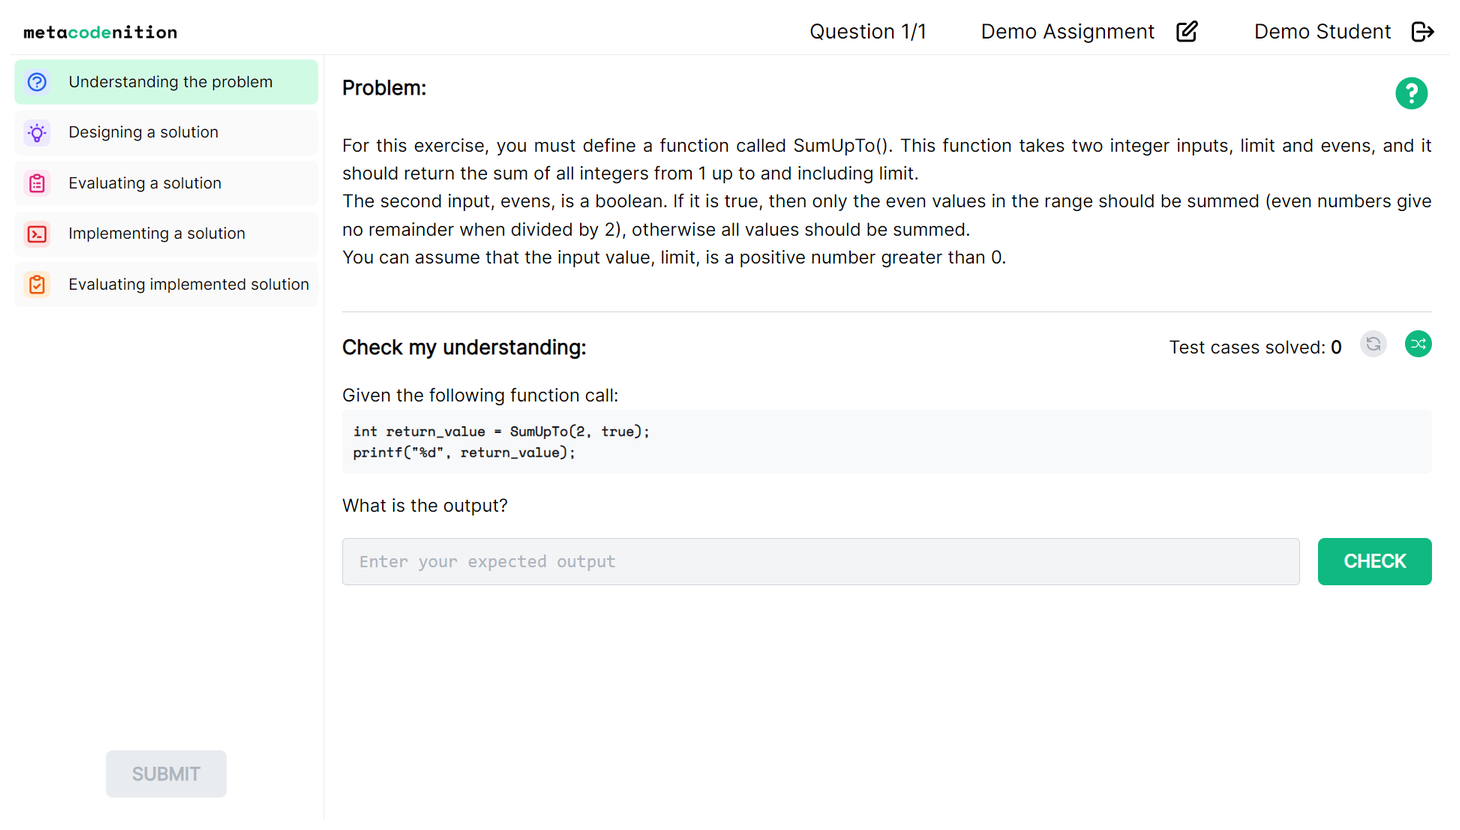
\includegraphics[width=\linewidth]{understanding-the-problem}
  \caption{Understanding the problem page.}
  \Description{A screenshot of Metacodenition's understanding the problem page.}
  \label{fig:understanding}
\end{figure*}





\section{Design} \label{sec:design}
Metacodenition is designed to provide scaffolding 
for the problem-solving framework proposed by Loksa et al. \cite{loksa20162}. The problem-solving interventions included in Metacodenition are inspired by existing literature in which positive effects have been demonstrated:
%which has shown positive results previously:
\begin{itemize}
\item solving test cases before programming \cite{craig2019, denny2019, prather2019},
\item design parsons problems \cite{garcia2021},
\item test-driven development for education \cite{janzen2008}.
\end{itemize}
Additionally, Metacodenition's design is informed by the design implications for problem-solving tools proposed by Sáenz and Russis \cite{saenz2022}. Specifically, the design implications we incorporate in Metacodenition are:
\begin{itemize}
\item supporting artefacts different from code,
\item integrate and link the programming exercise text to the code constructs,
\item formatting and commenting features for the text and code.
\end{itemize}

\subsection{Scaffolding} \label{sec:design-scaffolding}
Scaffolding for the problem-solving steps should be presented in a logical order. Loksa et al.'s problem-solving stages are intended to be visited in a loose sequential manner. Stages should be revisited often while iteratively implementing a solution. Metacodenition provides the scaffolding for the problem-solving steps in a navigation bar, which shows all stages in order from top to bottom, with the current stage being highlighted. This is designed to help the student visualise their problem-solving state. 

Upon opening a new programming assignment, or moving to the next question within an assignment, the user is navigated to the first stage. Students can freely visit stages, allowing them to revisit previous stages or skip ahead as needed.
%In the initial evaluation of Metacodenition that we present in Section \ref{sec:evaluation}, student participation with the different stages in the tool is ungraded. 
%We chose to make engagement with the tool optional. 
Students can skip specific interventions, problem-solving stages, questions, or even assignments. 
This freedom is a deliberate design choice, and allows students to move through the tool and manage their own problem-solving process.

\subsection{Problem-solving stages} \label{sec:design-stages}
Metacodenition presents an adapted version of Loksa et al.'s problem-solving stages, more suitable for display in a navigation bar:
\begin{enumerate}
    \item reinterpreting the problem prompt \(\rightarrow \) understanding the problem,
    \item searching for solutions \(\rightarrow \) designing a solution,
    \item evaluating a potential solution \(\rightarrow \) evaluating a solution,
    \item implementing a solution,
    \item evaluating implemented solution
\end{enumerate}

We chose not to support Loksa et al.'s stage 2, \emph{searching for analogous problems} because Metacodenition was designed to be used 
%in a single lab. 
by novices with little to no prior programming experience. 
In Loksa et al.'s study, students are introduced to the stages through a lecture, while Metacodenition is designed to be used standalone, so we shortened the names of some stages to be more intuitive. Stages (1) and (2) are renamed for simplicity, while stage (3) is renamed to be concise.

A problem-solving tool should support artefacts different from code \cite{saenz2022}; therefore, we capture students' solutions to activities for each stage in Metacodenition, not just their final solution.

\subsection{Interventions} \label{sec:design-interventions}
\subsubsection{Understanding the problem} \label{sec:design-interventions-understanding}
The \emph{understanding the problem} stage is where a student should read and understand the problem. In Metacodenition, this stage consists of the problem description and an area to solve test cases, as shown in \autoref{fig:understanding}. The use of test case solving is informed by previous literature showing the benefits to problem comprehension of solving test cases before programming. The student is shown a function call and is asked to enter their expected output. They can check their answer using the \emph{Check} button or by pressing an enter key. Students can shuffle through test cases using the \emph{Shuffle} button if they get stuck on one test case for too long.

Test cases that the student solves are added to a bank of solved test cases that are later used in the \emph{Evaluating implemented solution} stage. The intention is to add an incentive for students to complete multiple test cases before they start programming, making it more likely that the student will discover flaws in their understanding of the problem before they write any code.


\subsubsection{Designing a solution} \label{sec:design-interventions-designing}
The \emph{designing a solution} stage is where a student reads through the problem and identifies programming constructs or patterns that they think may be relevant for solving parts of the problem. 
%programming patterns they have used or encountered in the past which may be relevant. 
\autoref{fig:designing} shows the \emph{designing a solution stage} on Metacodenition. A problem-solving tool should integrate and link the programming exercise text to the code constructs and have formatting and commenting features for the text and code \cite{saenz2022}. In Metacodenition, this is achieved by allowing the student to highlight parts of the problem text that they think require code to achieve, and then assign an action to them. By assigning an action to a part of the problem statement, the student identifies a programming pattern or code construct that they can use to address that part of the problem. For example, the student may identify that a modulo operator can be used (action) to check if a value is even (problem statement).

Everywhere that the problem statement appears in the IDE reflects the markup added in this stage. For example, if a student were to move back to the \emph{understanding the problem} stage, they would be able to see their highlighted problem statement. Further, hovering over a highlighted section of the problem statement would make a pop-up visible that contained the user’s action. This allows the student to quickly reference the problem and their actions from every page in the IDE.

\begin{figure}[h!]
  \centering
  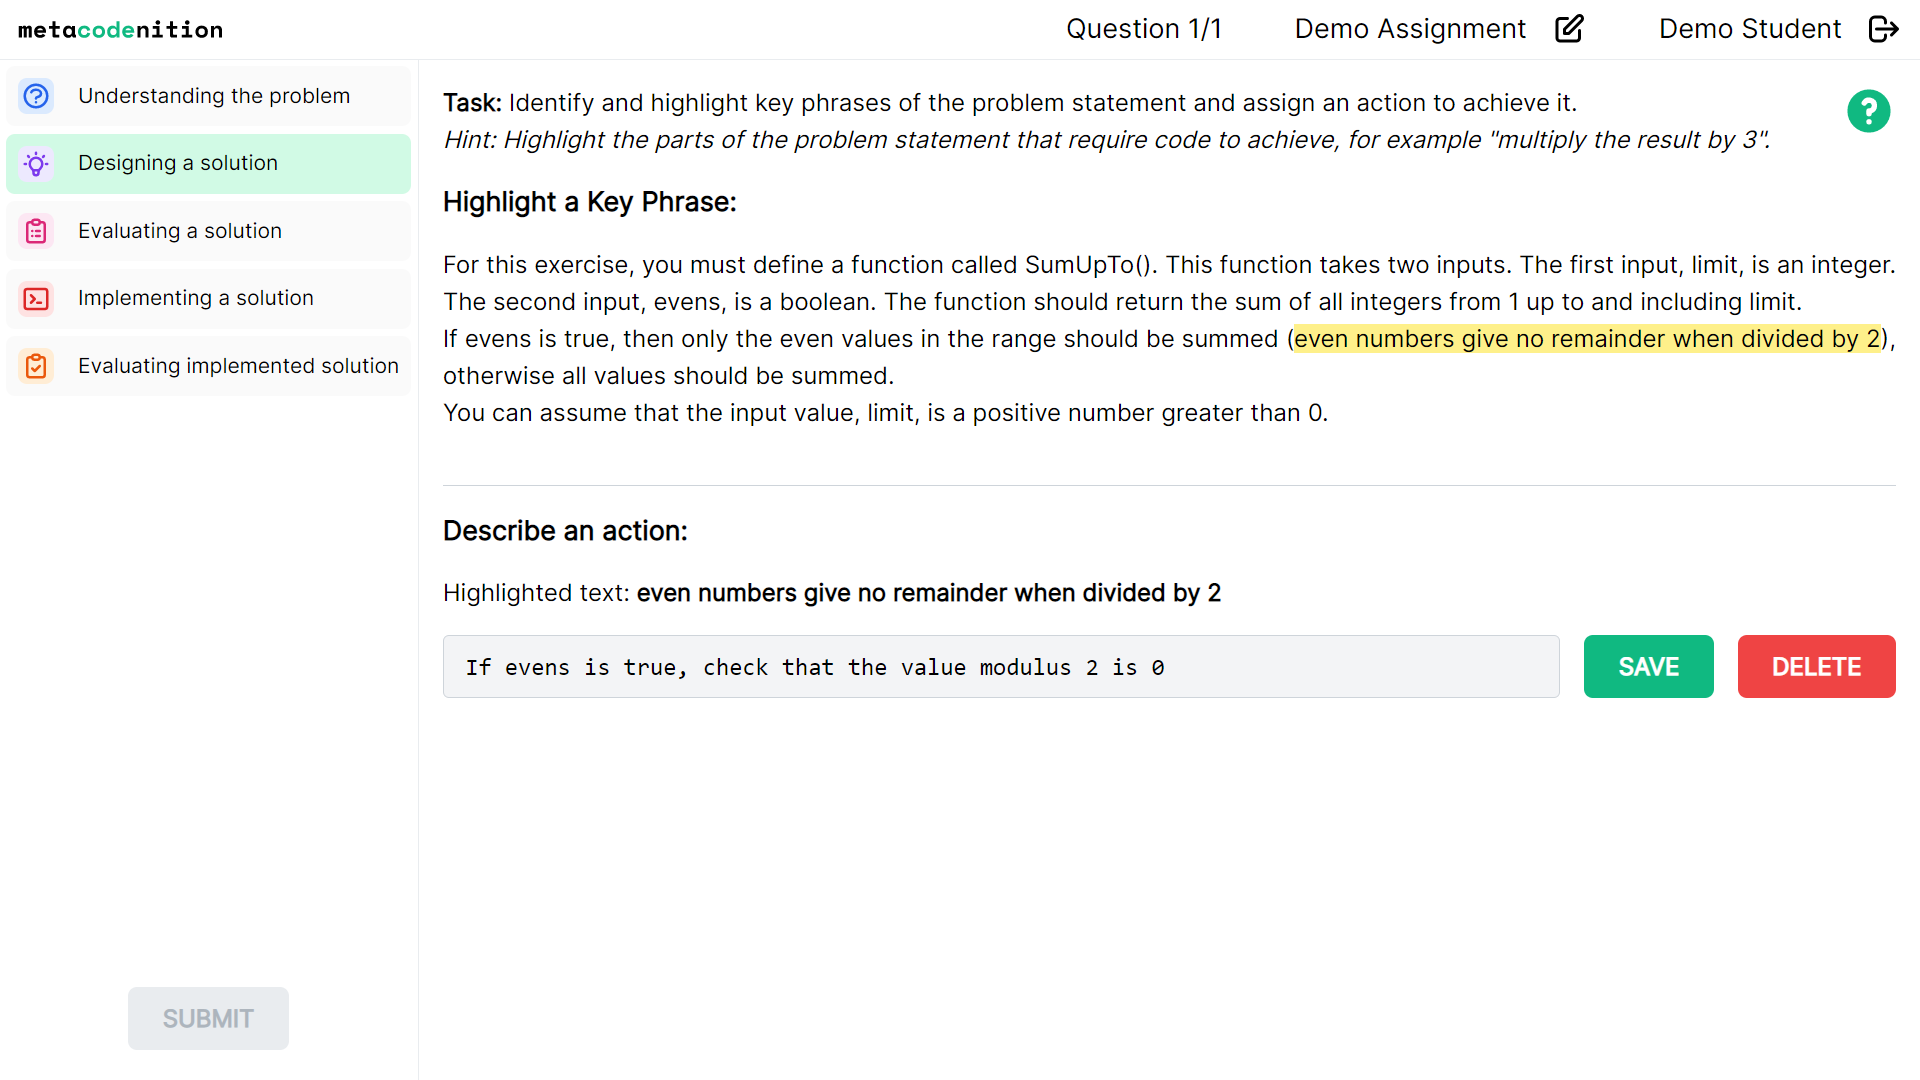
\includegraphics[width=\linewidth]{designing-a-solution}
  \caption{Designing a solution page.}
  \Description{A screenshot of Metacodenition's designing a solution page.}
  \label{fig:designing}
\end{figure}

\subsubsection{Evaluating a solution} \label{sec:design-interventions-evaluating}
The \emph{evaluating a solution} stage (see \autoref{fig:evaluating}) is where a student forms an action plan for their program by selecting and rearranging actions they created previously in the \emph{designing a solution} stage. Students can do this by dragging and dropping blocks from the \emph{My Actions} section to the \emph{My Action Plan} section. There is also functionality to create new actions if a student feels that the actions they generated previously are insufficient. Design Parsons problems inspire this stage \cite{garcia2021}, where instead of students being provided with fragments to rearrange, students use previously created fragments. In designing Metacodenition, we particularly wanted to have a strong interconnection of stages to support a good flow through the problem-solving process. Using users' previously created actions, we found a more suitable solution for our goal of interconnection than pre-defined fragments.

\begin{figure}[h!]
  \centering
  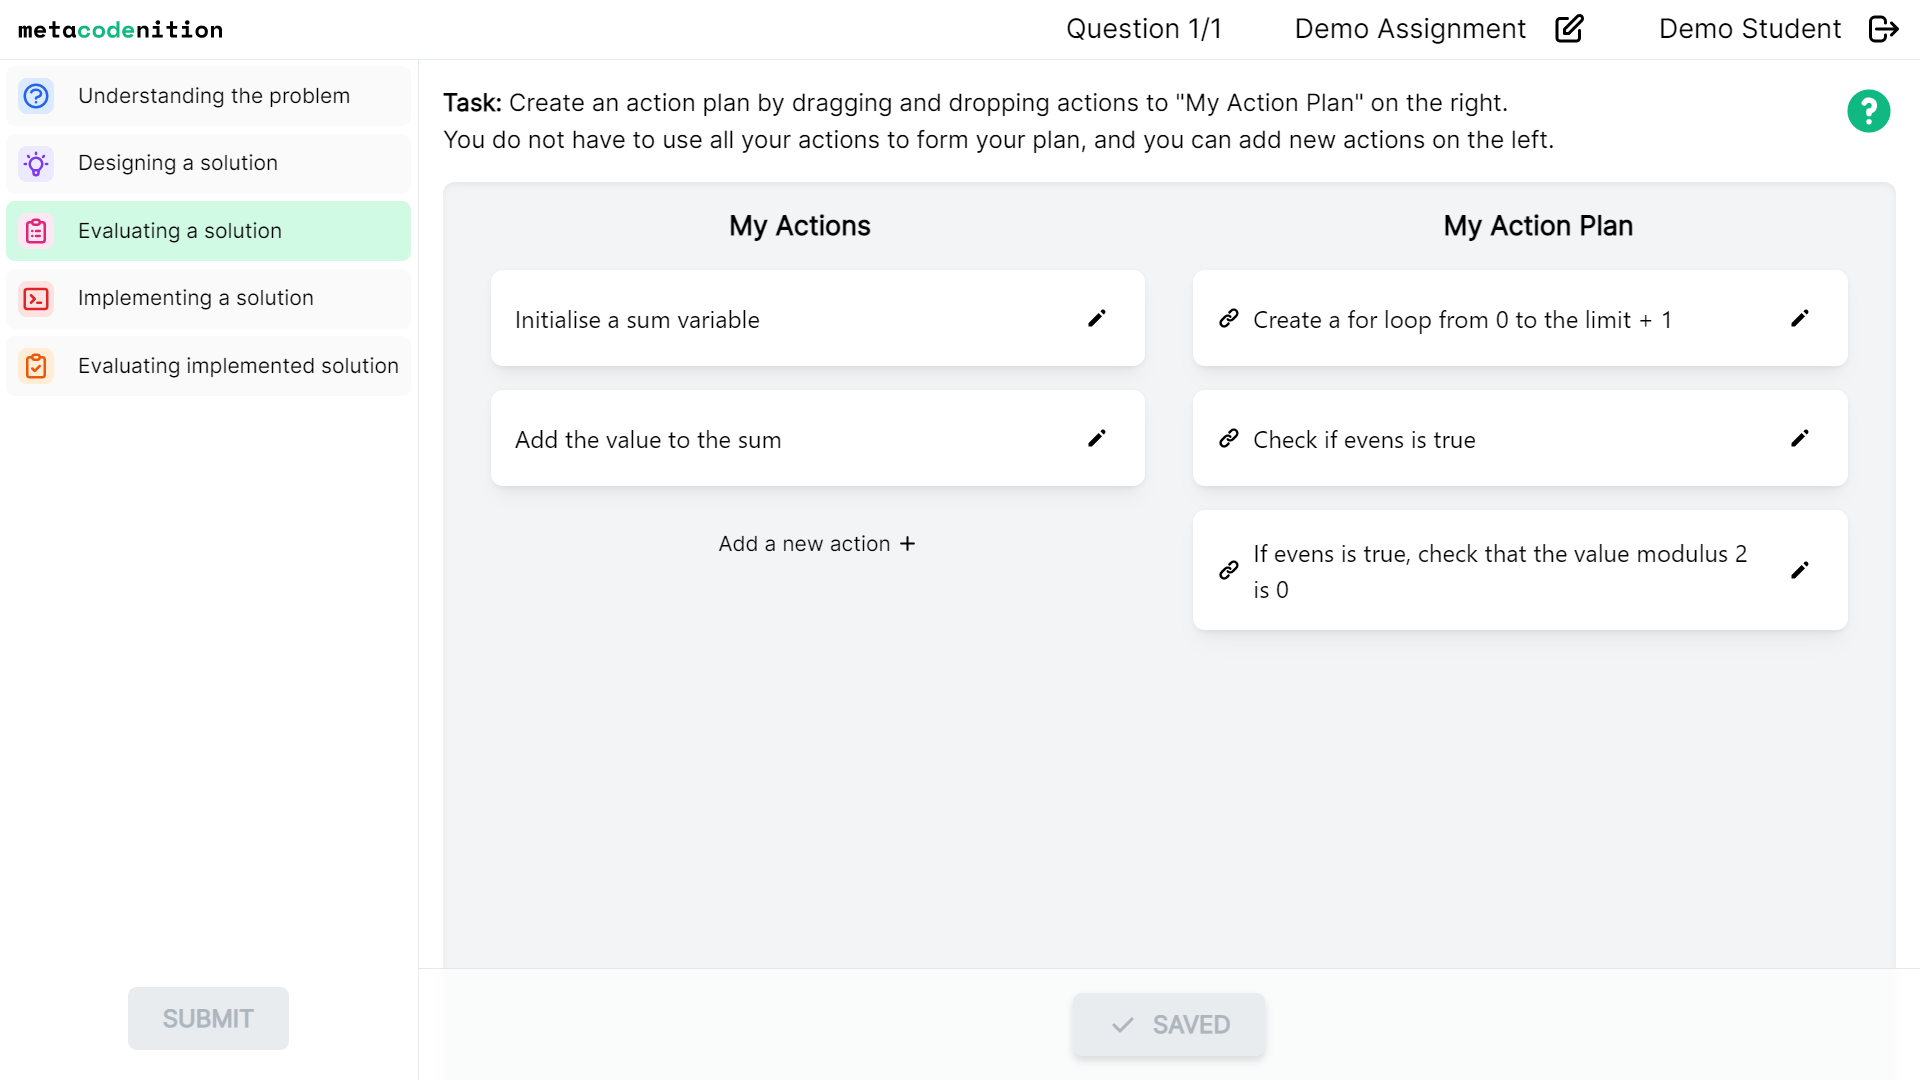
\includegraphics[width=\linewidth]{evaluating-a-solution}
  \caption{Evaluating a solution page.}
  \Description{A screenshot of Metacodenition's evaluating a solution page.}
  \label{fig:evaluating}
\end{figure}

\subsubsection{Implementing a solution} \label{sec:design-interventions-implementing}
The \emph{implementing a solution} stage is where students write their code, as shown in \autoref{fig:implementing}. This screen is split into two sections: an area to write their code and a panel with three different tabs. A problem-solving tool should integrate and link the programming exercise text to the code constructs \cite{saenz2022}, which we address in the page's tab design. Tab 1, the default tab, shows the previous action plan the student created, which can be used to inform their solution. Tab 2 shows the problem statement along with its highlights and assigned actions. Tab 3 is an area where students can run and debug their code.

\begin{figure}[h!]
  \centering
  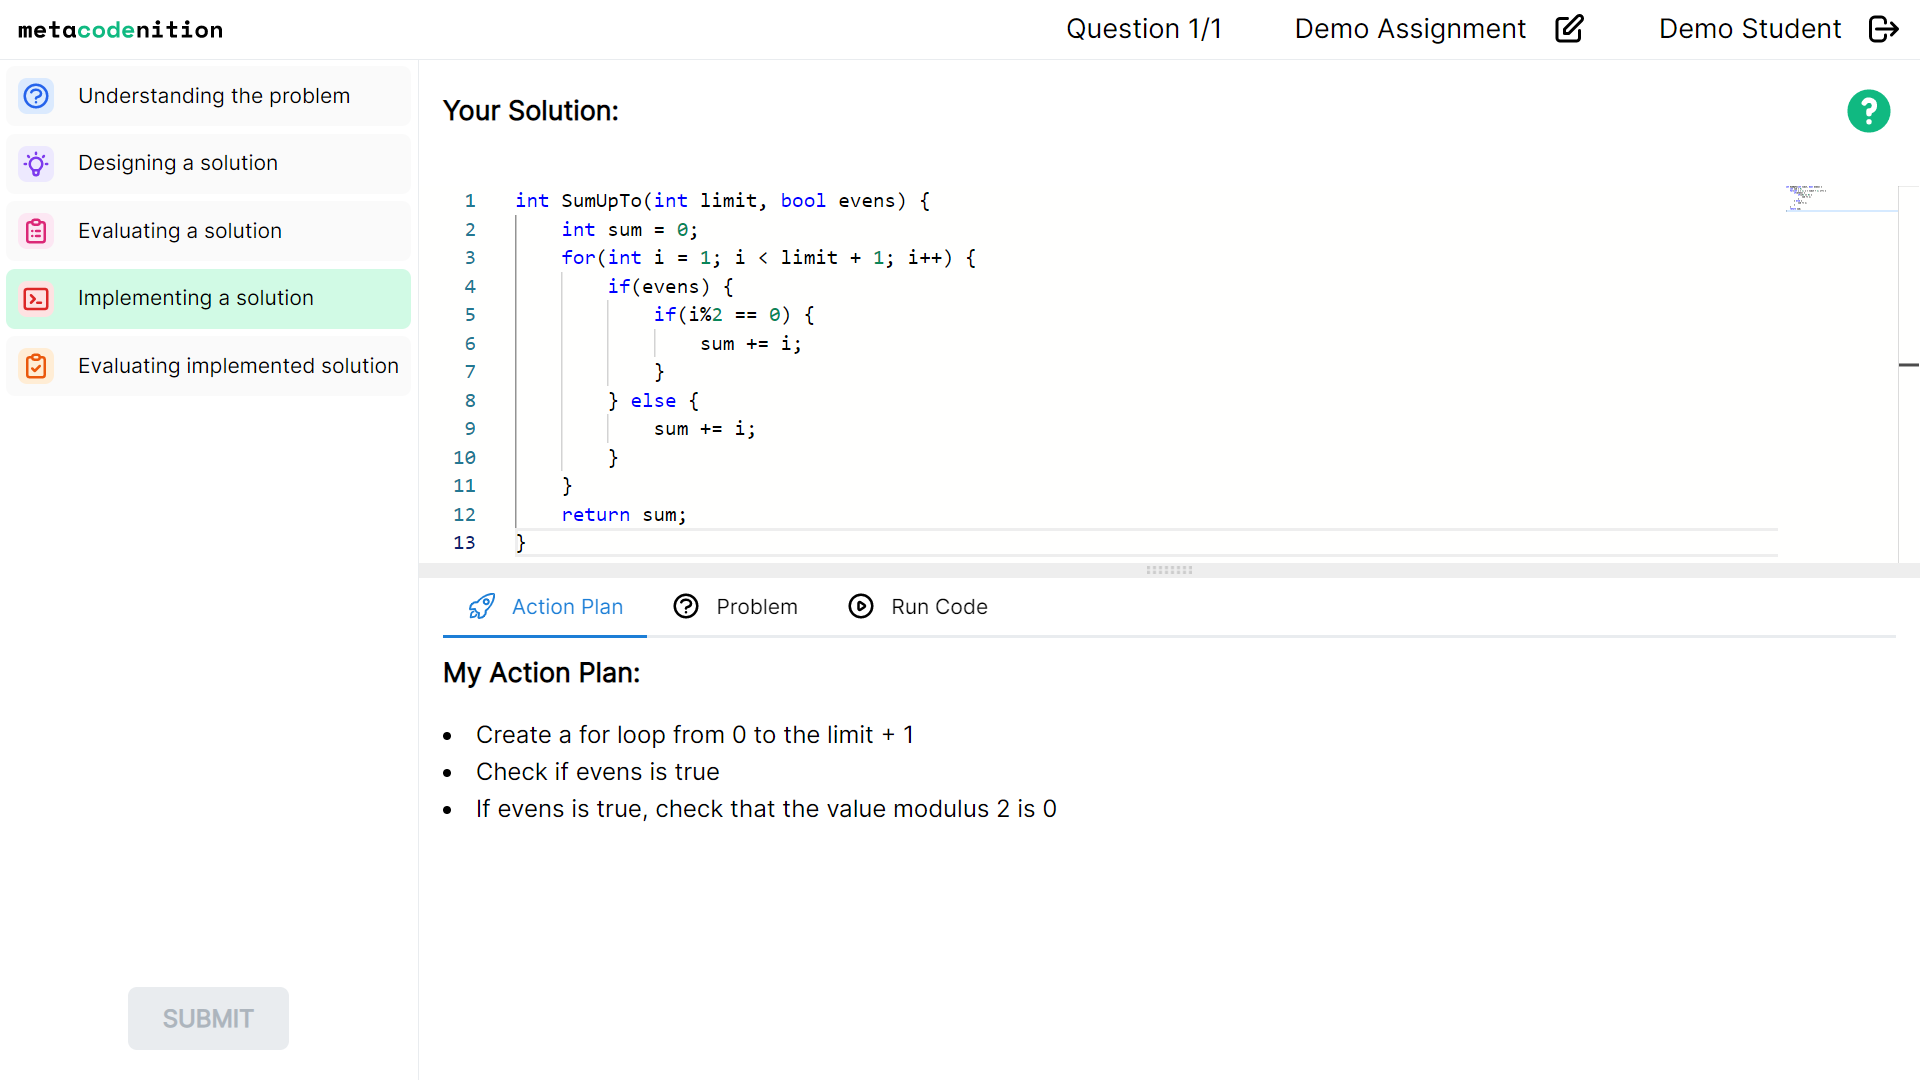
\includegraphics[width=\linewidth]{implementing-a-solution}
  \caption{Implementing a solution page.}
  \Description{A screenshot of Metacodenition's implementing a solution page.}
  \label{fig:implementing}
\end{figure}

\subsubsection{Evaluating implemented solution} \label{sec:design-interventions-testing}
We provide a student-friendly testing interface in the \emph{evaluating implemented solution} stage. Students can test their code against test cases they previously solved in the \emph{understanding the problem} stage. Test cases they did not solve previously are disabled. Students also have the option to add their own test cases. Not all test cases used to grade the students' submissions were provided by Metacodenition as a means to incentivise students to define their own.

\autoref{fig:evaluatingimplemented} shows the user interface for this stage. The functionality of solving test cases before programming and then running these test cases after programming is inspired by test-driven development (TDD) \cite{janzen2008}. Like TDD, students convert requirements from the problem statement into test cases before developing and testing their solution against all test cases. The main difference is that the students' test suites are built by solving pre-defined test cases rather than writing their own. While traditional TDD for education has proven successful in isolation, Metacodenition provides multiple non-code-writing activities for students to complete. Consequently, keeping each activity short to minimise impedance becomes particularly important to keep students motivated. 

\begin{figure}[h!]
  \centering
  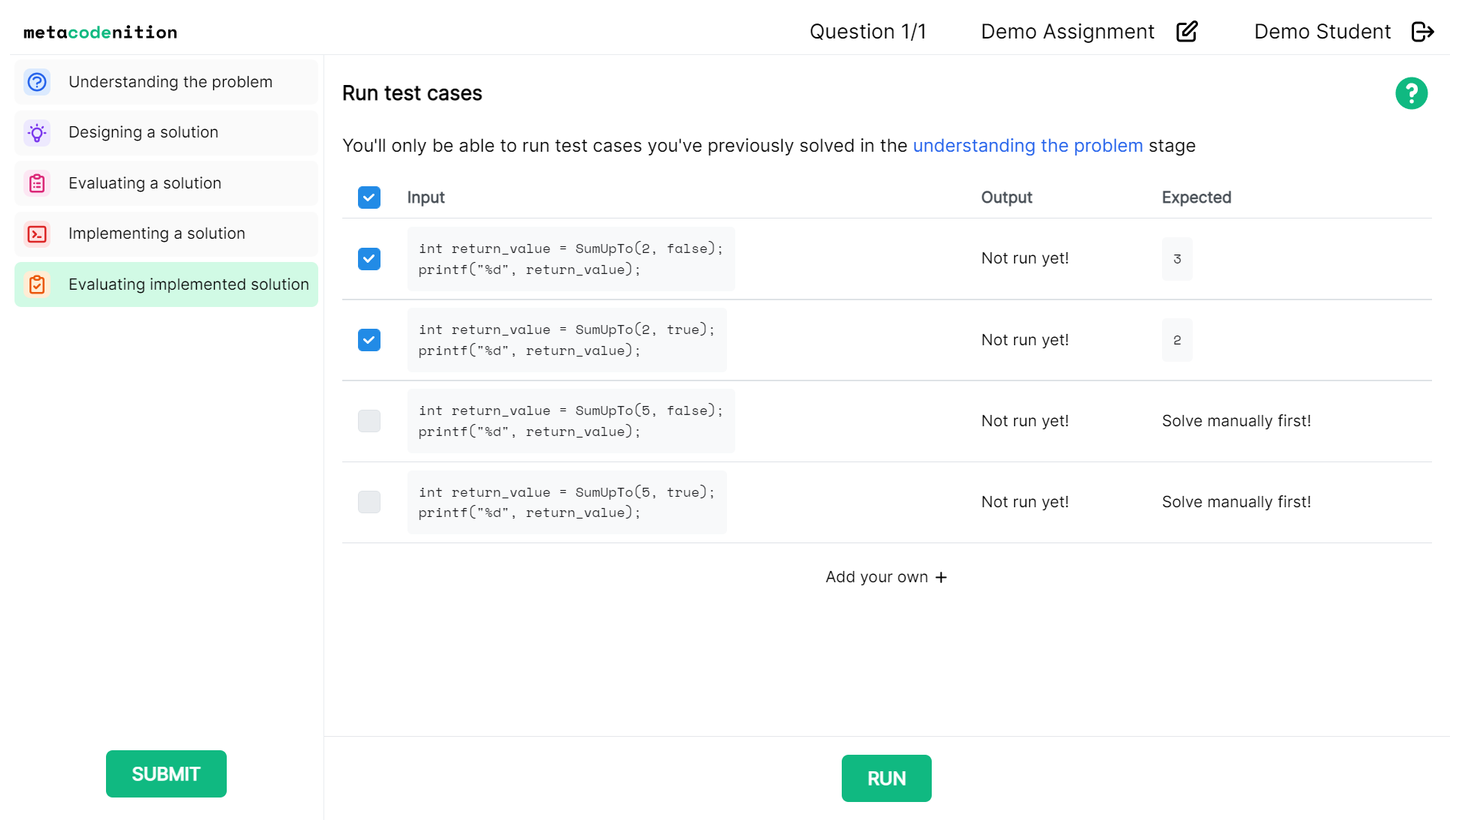
\includegraphics[width=\linewidth]{evaluating-implemented-solution}
  \caption{Evaluating implemented solution page.}
  \Description{A screenshot of Metacodenition's evaluating implemented solution page.}
  \label{fig:evaluatingimplemented}
\end{figure}

\section{Evaluation} \label{sec:evaluation}
Our evaluation of Metacodenition is guided by the two research questions in \autoref{sec:introduction}. These explore students' performance on code-writing tasks and their perceptions when using Metacodenition for problem-solving activities. We conducted an evaluation in a large first-year software engineering course at \{\emph{Institution anonymized for review}\}.
%the University of Auckland. 

For our evaluation, Metacodenition was used as a lab activity consisting of six problems, A-F, targeting loops and arrays in the C programming language. Problems A-C were completed by students in their own development environments and served as warm-up exercises. These problems ensured students were comfortable with the concepts required to answer problems D-F in Metacodenition. We refer to these three problems, answered in Metacodenition, as problems 1-3 in the rest of this paper. \autoref{tab:problems} displays the descriptions students were provided  for each of these problems.

\begin{table*}
  \caption{Table of Problems used in Metacodenition}
  \label{tab:problems}
  \begin{tabular}{c p{37em} p{14em}}
    \toprule
    \# & Problem Prompt & Interventions Active\\
    \midrule
    1 &Define a function called SumPositiveValues() which is passed two inputs: an array of integers, and an integer indicating how many elements are in the array. The function should return the sum of all positive integers in the input array.& Group A: All\newline Group B: Implementing a Solution\\
    \midrule
    2 &Define a function called PrintSummary() which is passed one input: an array of integers of unknown length. This function should determine whether there are more positive or more negative values in the array. You should only examine values in the array until the first occurrence of the value 0. If there are more positive than negative values, you should print the word "Positive". If there are more negative values than positive values, you should print the word "Negative". If there are an equal number of positive and negative values, you should print the word "Equal".& Group A: Implementing a Solution\newline Group B: All\\
    \midrule
    3 &Define a function called PrintAverageRainfall() which is passed an array of integers representing daily rainfall amounts. The function should calculate and print the average rainfall. The daily rainfall amounts are occasionally corrupted, represented by negative values, so any negative value should be ignored from your calculation. The array also contains a special value, -999, to indicate the end of the valid rainfall data, so you should only examine values in the array up to the first occurrence of the value -999. Print the average of the valid rainfall data, rounded to 2d.p. For example, if there is just one valid rainfall value of 1, then the output of the function should be "1.00". If there are no valid rainfall values then print "no rain". & Group A: Free Choice\newline Group B: Free Choice\\
  \bottomrule
\end{tabular}
\end{table*}

\subsection{User groups} \label{sec:evaluation-usergroups}
To address our research question about the effect of scaffolding on students' performance on code-writing tasks, we 
randomly assigned students to one of two groups (A or B) at the time they logged in to 
%split students into one of two user groups (A or B) when they logged in to 
Metacodenition. In \autoref{sec:results-testcases}, we describe the measures we use for performance. Of the 821 students who used Metacodenition, 392 were in group A, and 429 were in group B.

For Problem 1, students in Group A were given access to all of the problem-solving stages within Metacodenition, while students in Group B were given access only to the \emph{implementing a solution} stage. For Problem 2, these conditions switched and students in Group A were given access to only the \emph{implementing a solution} stage, and students in Group B were given access to all stages. For the Problem 3, students were prompted to select which of the problem-solving stages they wished to enable before starting the problem. The interventions available to students in each group for each problem are summarised in \autoref{tab:problems}.

We have excluded Problem 3 from the analysis we present here because for this problem both user groups were able to select the interventions that were active. We hypothesise that students will perform better when answering problems with all interventions activated.  We explore student performance on Problems 1 and 2 to test this hypothesis with respect to RQ2.

\subsection{Questionnaire} \label{sec:evaluation-questionnaire}
At the end of the lab, an optional questionnaire was displayed for students to answer. The following questions were asked to address RQ1 regarding student perceptions of Metacodenition:
\begin{enumerate}
    \item How helpful was the problem-solving assistance?
    \item Which assistance was the most helpful?
    \item I would use this tool again if it was optional (True or False).
    \item What worked well?
\end{enumerate}
Question 1 was a five-point scale question that asked students to rank how easy it was to use Metacodenition from zero (extremely difficult) to five (extremely easy). Question 2 was close-ended, allowing students to select a problem-solving stage. Question 3 was a close-ended question presented as a checkbox, allowing students to check if they agreed with the statement. Question 4 was an open-ended question intended to collect student anecdotes.

The questionnaire also included several questions to identify room for improvement or to report any bugs that students encountered:
\begin{itemize}
    \item How easy was it to use this tool?
    \item What went wrong?
\end{itemize}

\begin{figure}[h!]
  \centering
  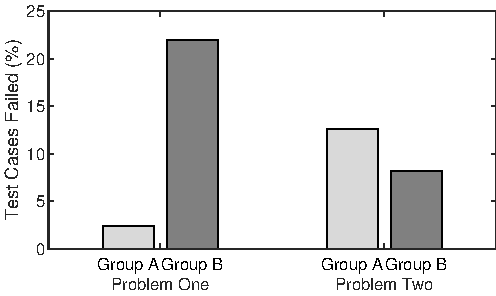
\includegraphics[width=\columnwidth]{test_cases}
  \caption{Percentage of test cases failed for final submissions per user group per question.}
  \Description{A bar graph showing the percentage of test cases failed in final submissions per user group per question.}
  \label{fig:testcases}
\end{figure}


\section{Results and Discussion} \label{sec:results}
\subsection{Test cases failed in final submissions} \label{sec:results-testcases}
The metric we used to measure a group's performance was the percentage of test cases that all of a group's final submissions failed. Each student could run their solution as often as they would like, but they could not go back and change their solution after moving to the next problem. Their solution when they move to the next question forms their final submission and reflects the solution which they believe is complete. We ran all final submissions against a test suite, which consisted of the test cases available to students in the \emph{evaluating implemented solution} stage. We also included ``hidden'' test cases in our suite, which were additional test cases not presented to students in the tool. \autoref{tab:test_cases} presents the number of test cases failed for Problems 1 and 2 by user group.


%KEITH!!!  We are almost there!
%% We only need a few lines now.  I will abbreviate some of the text in the references: like Proceedings -> Proc
%% It will take me 5 mins
%% In the meantime, if you have spare time, please just do a quick top to bottom check. 
%%...oh let me read your commetn above. 
%% Yeah, I liked it better before because it was very explicit.  Go ahead and put it back and I'll still look to save space elsewhere. 


%% I'll be in the bib file.
\begin{table}
\footnotesize
\caption{Test cases failed in final submissions for Problems 1 and 2.}
  \label{tab:test_cases}
  \begin{tabular}{c|c|c|c}
    \toprule
    \multirow{2}{*}{Problem \#} & \multirow{2}{*}{Hidden (Y/N)} & \multicolumn{2}{c}{Failed Count} \\
    \cmidrule{3-4}
      &   & A & B \\
    \midrule
    \multirow{10}{*}{1}& N & 7 & 20 \\
    \cmidrule{2-4}
    & N & 7 & 25 \\
    \cmidrule{2-4}
    & N & 8 & 23 \\
    \cmidrule{2-4}
    & N & 9 & 124\\
    \cmidrule{2-4}
    & N & 9 & 125\\
    \cmidrule{2-4}
    & N & 10 & 124\\
    \cmidrule{2-4}
    & Y & 11 & 125\\
    \cmidrule{2-4}
    & Y & 11 & 124\\
    \cmidrule{2-4}
    & Y & 10 & 125 \\
    \cmidrule{2-4}
    & Y & 11 & 125\\
    \midrule
    \multirow{12}{*}{2} & N & 46 & 32 \\
    \cmidrule{2-4}
    & N & 46 & 34 \\
    \cmidrule{2-4}
    & N & 49 & 34 \\
    \cmidrule{2-4}
    & N & 47 & 33\\
    \cmidrule{2-4}
    & N & 50 & 34\\
    \cmidrule{2-4}
    & N & 50 & 37\\
    \cmidrule{2-4}
    & Y & 52 & 32\\
    \cmidrule{2-4}
    & Y & 50 & 36\\
    \cmidrule{2-4}
    & Y & 50 & 37 \\
    \cmidrule{2-4}
    & Y & 51  & 35\\
    \cmidrule{2-4}
    & Y & 46 & 33 \\
    \cmidrule{2-4}
    & Y & 53 & 36 \\
  \bottomrule
\end{tabular}
\end{table}

\autoref{fig:testcases} shows the percentage of test cases that failed in final submissions per user group per problem. We see that for Problem 1, the percentage of test cases failed by Group A, which received scaffolding for this problem, is approximately 2\%, compared to approximately 22\% by Group B. For Problem 2, where the scaffolding was switched between groups, the percentage of test cases failed by Group B is approximately 8\%, in contrast to approximately 13\% by Group A. The switching of these results show that students who receive all scaffolding tend to fail fewer test cases than students who receive no scaffolding. On the surface, this could be attributed to students who received all interventions having the ability to view the non-hidden cases in the test suite (understanding the problem) and test their code against them  (evaluating implemented solution) before submission. However, as we see in \autoref{tab:test_cases}, this trend still holds for \emph{hidden} test cases, which were not available to either group. 
%Additionally, students could still manually run test cases when they did not have scaffolding. The difference is that when students had scaffolding, they were explicitly prompted to run their code against test cases. When they did not have scaffolding, they were not made aware of their problem-solving state or the corresponding actions to take. 
Additionally, students could still manually run test cases when they did not have scaffolding, they just weren't explicitly prompted to do so. 
This indicates that Metacodenition's scaffolding positively affects test case failure rates. We also see that the gap between the percentage of failed test cases is smaller for Problem 2 than for Problem 1. A possible explanation is that the group of students who did not receive scaffolding for Problem 2, but had previously received scaffolding for Problem 1, had better metacognitive awareness of the value of testing as part of the problem-solving process. 
%Hence, they self-initiated the task of running test cases.


\subsection{Student perceptions of Metacodenition's scaffolding} \label{sec:results-questionnaire}
Most students found the scaffolding provided by the \emph{evaluating implemented solution} stage the most helpful. The second most helpful stage deemed by students was the \emph{understanding the problem} stage. \autoref{fig:interventions} presents the number of students who indicated each stage to be the most helpful. It is no surprise that students found \emph{evaluating implemented solution} to be the most helpful, as this stage appears to contribute the most to the final solution. The popularity of \emph{understanding the problem} is also expected, as this intervention is supported by past studies showing positive results. Still, we view it as a strong result that this stage was well received by students when combined with the other scaffolding in Metacodenition, as prior  work has only  studied its effects in isolation.

\begin{figure}[h!]
  \centering
  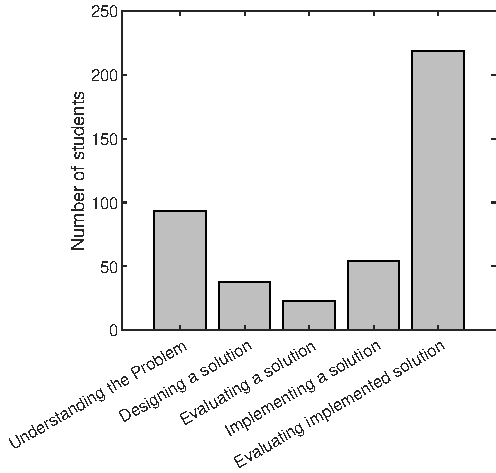
\includegraphics[width=\columnwidth]{intervention_responses}
  \caption{Responses to "Which assistance was the most helpful?".}
  \Description{A bar graph showing responses to the "Which assistance was the most helpful?" in the questionnaire.}
  \label{fig:interventions}
\end{figure}

\autoref{fig:usefulness} shows student responses to ``How helpful was the problem-solving assistance?''. The mean rating is approximately 3.18 out of 5, which corresponds to ``helpful''. Of the 427 students who answered the questionnaire, 304 (71\%) agreed with the statement, ``I would use this tool again if it were optional''. Together, these results indicate that most students perceived Metacodenition as a helpful tool they would use again, even if not required.

\begin{figure}[h!]
  \centering
  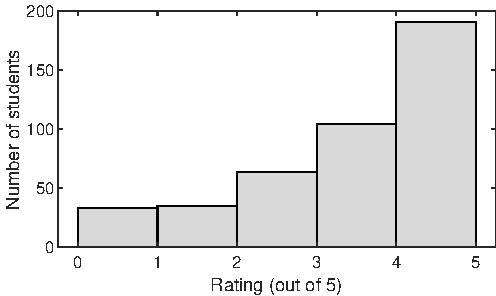
\includegraphics[width=\columnwidth]{usefulness_responses}
  \caption{Responses to ``How helpful was the problem-solving assistance?''.}
  \Description{A bar graph showing responses to the ``Which assistance was the most helpful?'' in the questionnaire.}
  \label{fig:usefulness}
\end{figure}

In the open-ended responses for ``What worked well?'', many students expressed that they particularly liked a certain stage of Metacodeniton:
\begin{itemize}
    \item ``Understanding the problem was a huge help. Not only did it allow for easy testing later but often there is a bit of ambiguity of what to do in a specific case so its really nice to have that sorted before I started coding.''
    \item ``I liked the Test cases and the highlighting of the question sections. I found I fully understood all the edge cases and sentences in the question that I would typically miss.''
%     \item ``Requiring the user to highlight and explain parts of the brief makes it much easier to make a pseudo code.''
     \item ``It was exactly like writing a pseudocode, except you could change the order of your plan easily. It was just super helpful to type down notes and clear my head before I started coding.''
    \item ``I really liked how I could write out a solution plan which outlined what I needed to do, and how it remained visible as I was writing my code.''
    \item ``I found the evaluating part helpful as it allowed me to see all the tests together and see patterns in the tests that failed.''
\end{itemize}

Other students indicated that they particularly liked how the \emph{understanding a problem} and \emph{evaluating implemented solution} stages linked together:
\begin{itemize}
    \item ``It was good to be able to manually solve the expected outputs and then test my code on those same test cases.''
    \item ``I like how we are able to check our code solution to something we hand worked first.''
    \item ``Manually working out answers and then comparing them to the code's actions was very useful.''
\end{itemize}


In Metacodenition, students were only shown the unedited messages from the compiler and multiple students expressed an interest in seeing better error reporting.  This supports the need for continued work on improving compiler error messages for novices.  One student stated: ``Some of the error messages are vague or hard to understand to inexperienced coders''.  
%Multiple students expressed interest in enhanced compiler error messages (ECEMs), with one stating: ``Some of the error messages are vague or hard to understand to inexperienced coders''. Multiple students indicated an interest in a specific ECEM, which is being informed when their code enters an infinite loop:
%\begin{itemize}
%    \item ``If a while loop prints something infinitely, it makes the output text box stretch out.''
%    \item ``Occasionally when my code didn't work, it didn't produce any output or give any error message so it was hard to move further.''
%\end{itemize}
In a similar vein, some students felt that they were missing some features from their usual IDE:
\begin{itemize}
    \item ``Actually using the page to code felt foreign and lacked many of the little errors coding in something in visual studio would pick up.''
    \item ``I personally find it easier overall to use downloaded ide like visual studio code.''
\end{itemize}

This feedback is likely because Metacodenition's code editor did not include a language server, one of the major features of modern IDEs. Language servers can provide in-editor error messages before compilation, or indexing the codebase, making navigation much easier. Many language servers also provide automatic code completion. Many of these features would likely be very useful for novice programmers as they are new to the syntax and semantics of writing code. However, language server error messages usually mirror compiler error messages, which are unhelpful to novices \cite{prather2017}.

Interestingly, one student responded, ``Felt like learning a new skill'' to the question on what went wrong. Though this student appears to have felt that something went wrong, we view their response as a positive indicator that Metacodenition achieved what we intended it to do -- which is to teach students problem-solving skills.

\subsection{Limitations} \label{sec:results-limitations}
One limitation, especially with respect to the development of metacognitive skills, is the limited time frame of our evaluation.  This evaluation was conducted as one lab activity in the course, which most students completed in a single sitting of roughly 30 minutes. Problem-solving skills take time to develop, so a longer time frame is needed to evaluate the effect of Metacodenition's interventions more robustly. Future studies should investigate these benefits over an extended period, such as an entire semester.

The problems employed in the lab were short and simplistic. They directly prescribed many of the actions students should take, which will have impacted the usefulness of Metacodenition. We also hypothesise that this would have skewed the results for students' preferred interventions, as there is relatively little to do in the \emph{designing a solution} and \emph{evaluating a solution} stages for these problems.

\section{Conclusions} \label{sec:conclusion}
This paper presents our approach to designing and evaluating a tool for novice programmers called Metacodenition, which provides metacognitive scaffolding for Loksa et al.'s problem-solving framework \cite{loksa20162}. By scaffolding the problem-solving process from start to finish, Metacodenition aims to explicitly promote the development of problem-solving skills in novices. Results from our initial evaluation show fewer test cases failed in the final submissions of students who received all of Metacodenition's scaffolding when compared to students who received only the \emph{implementing a solution} stage. We also found that most students perceived Metacodenition as a helpful tool they would voluntarily use in the future. 

Student feedback has highlighted a potential direction for improving Metacodenition, specifically in adding better support for error reporting.
%enhanced compiler error messages. 
Adding a ``pedagogic language server'' could also be helpful, providing enhanced compiler error messages in real-time as the student writes their code. 
Loksa et al.'s problem-solving framework also includes the \emph{searching for analogous problems} stage that Metacodenition currently omits. Here, students draw upon problems they have encountered previously, and additional future work could include adding an intervention for this stage. We suggest a ``problem bank'' of past problems a student has solved along with their solutions, allowing them to filter and identify relevant problems with similar patterns.

\bibliographystyle{ACM-reference-format}
\bibliography{sample-base}

\end{document}
\endinput
%%
%% End of file `sample-authordraft.tex'.
